\chapter{Operations and constructions over Vector Boolean Functions}

In this chapter, some basic constructions for Vector Boolean functions supported by the VBF
class are described. Some of them correspond to secondary
constructions, which build $(n,m)$ variable vector Boolean functions from
$(n',m')$ variable ones (with $n' \leq n, m' \leq m$). The direct sum has been
used to construct resilient and bent Boolean functions
 \cite{Carlet:04}. The concatenation can be used to obtain resilient functions or functions with maximal nonlinearity. The concatenation of polynomials in ANF can be used to obtain functions of high nonlinearity with $n$ variables from functions with high nonlinearity with $n'$ variables ($n' < n)$. Adding coordinate functions and bricklayering are constructions
used to build modern ciphers such as CAST \cite{CAST:256},  DES \cite{DES:77}
and AES \cite{DaemenR:02}. Additionally, VBF provides operations for
identification if two vector Boolean functions are equal, the sum of two
vector Boolean functions, the composition of two vector Boolean functions and the inverse of a Vector Boolean function.  

\section{Equality Testing}

\subsection{Description}

\begin{definition}
Let $n \geq 1, m \geq 1$, $F,G \in \funct{F}_{n,m}$. $F$ and $G$ are \textit{equal} if their Truth Tables are the same.   
\end{definition}

\subsection{Library}

We can compare two functions for equality with the following method: 

\begin{verbatim}
long operator==(VBF& F, VBF& G)
long operator!=(VBF& F, VBF& G)
\end{verbatim}

\begin{example}
The following program informs if two Vector Boolean functions are equal given their Truth Tables.

\begin{verbatim}
#include <iostream>
#include <fstream>
#include "VBF.h"

int main(int argc, char *argv[])
{
   using namespace VBFNS;

   VBF          F, G, X;
   NTL::mat_GF2 Tf, Tg;

   ifstream input1(argv[1]);
   if(!input1) {
      cerr << "Error opening " << argv[1] << endl;
      return 0;
   }
   input1 >> Tf;
   F.puttt(Tf);
   input1.close();

   ifstream input2(argv[2]);
   if(!input2) {
      cerr << "Error opening " << argv[2] << endl;
      return 0;
   }
   input2 >> Tg;
   G.puttt(Tg);
   input2.close();

   if (F == G) {
     cout << "F and G are equal" << endl;
   }  else {
     cout << "F and G are not equal" << endl;
   }
   
   return 0;
}
\end{verbatim}

The output for the execution of the example program with the code above and the Truth Tables of $S_1$ and $S_2$ DES S-boxes as inputs would be:

\begin{verbatim}
F and G are not equal
\end{verbatim}
\end{example}

\section{Composition Function}\label{sec:Composition}

\subsection{Description}

\begin{definition}
Let $F \in \funct{F}_{n,p}$, $G \in \funct{F}_{p,m}$ and the composition function $G \circ F \in \funct{F}_{n,m}$ where $G \circ F (\vec{x}) = G (F(\vec{x})) \ \fa \vec{x} \in \gf{V_n}$. See figure~\ref{fig:Composition}.
\end{definition}

\begin{figure}[htbp!]
\centering
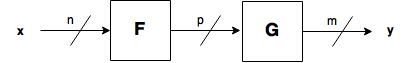
\includegraphics{Composition}
\caption[Composition]{\textit{Composition}.}
\label{fig:Composition}
\end{figure}

\subsection{Library}

It can be obtained with the following method:

\begin{verbatim}
void Comp(VBF& X, VBF& F, VBF& G)  
\end{verbatim}  

\begin{example}
The following program provides the correlation immunity and balancedness of two Vector Boolean functions given their Truth Tables and calculates the same criteria for their composition.

\begin{verbatim}
#include <iostream>
#include <fstream>
#include "VBF.h"

int main(int argc, char *argv[])
{
   using namespace VBFNS;

   VBF          F, G, X;
   NTL::mat_GF2 Tf,Tg;

   ifstream input1(argv[1]);
   if(!input1)  {
      cerr << "Error opening " << argv[1] << endl;
      return 0;
   }
   input1 >> Tf;
   F.puttt(Tf);
   input1.close();

   ifstream input2(argv[2]);
   if(!input2) {
      cerr << "Error opening " << argv[2] << endl;
      return 0;
   }
   input2 >> Tg;
   G.puttt(Tg);
   input2.close();

   cout << "Correlation immunity of F: " << CI(F) << endl;
   if (Bal(F)) {
     cout << "F is a balanced function" << endl;
   } else {
     cout << "F is a non-balanced function" << endl;
   }
   cout << endl;

   cout << "Correlation immunity of G: " << CI(G) << endl;
   if (Bal(G)) {
     cout << "G is a balanced function" << endl;
   } else {
     cout << "G is a non-balanced function" << endl;
   }
   cout << endl;

   Comp(X,F,G);

   cout << "Correlation immunity of GoF: " << CI(X) << endl;
   if (Bal(X)) {
     cout << "GoF is a balanced function" << endl;
   } else {
     cout << "GoF is a non-balanced function" << endl;
   }

   return 0;
}
\end{verbatim}

If we use $\vec{y_0}$ of CLEFIA $S_0$ cipher (see section "Analysis of CRYPTEC project cryptographic algorithms") and $NibbleSub$ Truth Tables as inputs, the output would be the following:

\begin{verbatim}
Correlation immunity of F: 1
F is a balanced function

Correlation immunity of G: 0
G is a balanced function

Correlation immunity of GoF: 1
GoF is a balanced function
\end{verbatim}

\end{example}

\begin{example}
The following program provides the balancedness of two Vector Boolean functions given its polynomial representation in ANF and calculates the balancedness for the its composition.

\begin{verbatim}
#include <iostream>
#include <fstream>
#include "VBF.h"

int main(int argc, char *argv[])
{
   using namespace VBFNS;

   VBF          F, G, X;
   vec_pol f,g;

   ifstream input1(argv[1]);
   if(!input1)  {
      cerr << "Error opening " << argv[1] << endl;
      return 0;
   }
   input1 >> f;
   F.putpol(f);
   input1.close();

   ifstream input2(argv[2]);
   if(!input2) {
      cerr << "Error opening " << argv[2] << endl;
      return 0;
   }
   input2 >> g;
   G.putpol(g);
   input2.close();

   cout << "The polynomial in ANF of F is ";
   cout << endl;
   Pol(cout,F);

   if (Bal(F)) {
     cout << "F is a balanced function" << endl;
   } else {
     cout << "F is a non-balanced function" << endl;
   }
   cout << endl;

   cout << "The polynomial in ANF of G is ";
   cout << endl;
   Pol(cout,G);

   if (Bal(G)) {
     cout << "G is a balanced function" << endl;
   } else {
     cout << "G is a non-balanced function" << endl;
   }
   cout << endl;

   Comp(X,F,G);
   cout << "The polynomial in ANF of the composition of F and G is ";
   cout << endl;
   Pol(cout,X);

   if (Bal(X)) {
     cout << "GoF is a balanced function" << endl;
   } else {
     cout << "GoF is a non-balanced function" << endl;
   }

   return 0;
}
\end{verbatim}

If we use the Boolean functions of first example described in \cite{GuptaS:05} as inputs, the output would be the following:

\begin{verbatim}
The polynomial in ANF of F is
x1+x2+x1x3+x1x2x3
x2+x1x2+x2x3+x1x3+x1x2x3
F is a non-balanced function

The polynomial in ANF of G is
x1+x2
G is a balanced function

The polynomial in ANF of the composition of F and G is
x2x3+x1+x1x2
GoF is a balanced function
\end{verbatim}

If we use the Boolean functions of second example described in \cite{GuptaS:05} as inputs, the output would be the following:

\begin{verbatim}
The polynomial in ANF of F is
x3+x1x2+x1x2x3
x2+x3+x1x2+x2x3+x1x2x3
F is a non-balanced function

The polynomial in ANF of G is
x1x2
G is a non-balanced function

The polynomial in ANF of the composition of F and G is
x3
GoF is a balanced function
\end{verbatim}

\end{example}

\section{Functional Inverse}

\subsection{Description}

\begin{definition}
Let $n \geq 1$, $F \in \funct{F}_{n,n}$. $F^{-1}$ is the \textit{functional inverse} of $F$ if the composition of both functions results in the identity function. See figure~\ref{fig:Inverse}.
\end{definition}

\begin{figure}[htbp!]
\centering
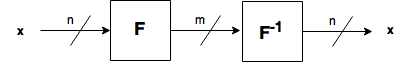
\includegraphics{Inverse}
\caption[Inverse]{\textit{Inverse}.}
\label{fig:Inverse}
\end{figure}

\subsection{Library}

If a Vector Boolean Function $F \in \funct{F}_{n,n}$ is invertible, then we can find its inverse with the following method:

\begin{verbatim}
void inv(VBF& X, VBF& F)
\end{verbatim}

\begin{example}
The following program provides the Truth Table of a the inverse of a Vector Boolean function given its Truth Table.

\begin{verbatim}
#include <iostream>
#include <fstream>
#include "VBF.h"

int main(int argc, char *argv[])
{
   using namespace VBFNS;

   VBF          F, X;
   NTL::mat_GF2 Tf;

   ifstream input1(argv[1]);
   if(!input1) {
      cerr << "Error opening " << argv[1] << endl;
      return 0;
   }
   input1 >> Tf;
   F.puttt(Tf);
   input1.close();

   inv(X,F);
   cout << "The Truth Table of the inverse of F is " << endl
   << TT(X) << endl;

   return 0;
}
\end{verbatim}

The output for the execution of the example program with the code above and the Truth Table of $NibbleSub$ S-box as input will be:

\begin{verbatim}
The Truth Table of the inverse of F is
[[1 1 1 0]
[0 0 1 1]
[0 1 0 0]
[1 0 0 0]
[0 0 0 1]
[1 1 0 0]
[1 0 1 0]
[1 1 1 1]
[0 1 1 1]
[1 1 0 1]
[1 0 0 1]
[0 1 1 0]
[1 0 1 1]
[0 0 1 0]
[0 0 0 0]
[0 1 0 1]
]
\end{verbatim}
\end{example}

\section{Sum}\label{sec:Sum}

\subsection{Description}

\begin{definition}
Let $n \geq 1, m \geq 1$, $F,G \in \funct{F}_{n,m}$. The \textit{Sum} of $F$ and $G$, denoted by $F + G \in \funct{F}_{n,m}$ 
is the Vector Boolean Function whose Truth Table results from the addition of the Truth Tables of $F$ and $G$: $\matr{T}_{F+G} = \matr{T}_F+\matr{T}_G$. 
\end{definition}

\subsection{Library}

It can be obtained with the following method:

\begin{verbatim}
void sum(VBF& X, VBF& F, VBF& G)  
\end{verbatim}

\begin{example}
The following program provides the nonlinearity, absolute indicator and linearity distance of two Vector Boolean functions given its polynomial representation in ANF and its hexadecimal representation of Truth Table respectively and calculates the same criteria for the its sum.

\begin{verbatim}
#include <iostream>
#include <fstream>
#include "VBF.h"

int main(int argc, char *argv[])
{
   using namespace VBFNS;

   VBF          F, G, X;
   vec_pol      f;

   ifstream input1(argv[1]);
   if(!input1)   {
      cerr << "Error opening " << argv[1] << endl;
      return 0;
   }
   input1 >> f;
   F.putpol(f);
   input1.close();

   ifstream input2(argv[2]);
   if(!input2)  {
      cerr << "Error opening " << argv[2] << endl;
      return 0;
   }
   G.putHexTT(input2);
   input2.close();

   cout << "The polynomial in ANF of F is ";
   cout << endl;
   Pol(cout,F);

   cout << "nl(F)=" << nl(F) << endl;
   cout << "ACmax(F)=" << maxAC(F) << endl;
   cout << "LD(F)=" << ld(F) << endl;
   cout << endl;

   cout << "The polynomial in ANF of G is ";
   cout << endl;
   Pol(cout,G);
   cout << endl;

   sum(X,F,G);
   cout << "The polynomial in ANF of the sum of F and G is ";
   cout << endl;
   Pol(cout,X);

   cout << "nl(F+G)=" << nl(X) << endl;
   cout << "ACmax(F+G)=" << maxAC(X) << endl;
   cout << "LD(F+G)=" << ld(X) << endl;
   cout << endl;

   return 0;
}
\end{verbatim}

If we use the Boolean function F with ANF $x_1x_2+x_3x_4$ and function G with hexadecimal representation of Truth Table $0001$ as inputs, the output would be the following:

\begin{verbatim}
The polynomial in ANF of F is
x1x2+x3x4
nl(F)=6
ACmax(F)=0
LD(F)=4

The polynomial in ANF of G is
x1x2x3x4

The polynomial in ANF of the sum of F and G is
x3x4+x1x2+x1x2x3x4
nl(F+G)=5
ACmax(F+G)=4
LD(F+G)=3
\end{verbatim}

These results are congruent with the properties of changing one bit of the Truth Table:

\begin{itemize}

\item $\crit{NL}(F+G)=\crit{NL}(F)-1=6-1=5$.

\item $\crit{AC_{max}}(F+G)=\crit{AC_{max}}(F)+4=0+4=4$.

\item $\crit{LD}(F+G)=\crit{LD}(F)-1=4-1=3$.

\end{itemize}

\end{example}

\section{Direct Sum}

\subsection{Description}

\begin{definition}
Let $n_1,n_2 \geq 1$, $F_1 \in \funct{F}_{n_1,m}, F_2 \in \funct{F}_{n_2,m}$ be Vector Boolean functions. Consider the Vector Boolean function $F_1 \oplus F_2 \in \funct{F}_{n_1+n_2,m}$, called direct sum, defined as $(F_1 \oplus F_2) \left( (\vec{x_1},\vec{x_2}) \right)= F_1(\vec{x_1}) + F_2(\vec{x_2})$. See figure~\ref{fig:DirectSum}.
\end{definition}

\begin{figure}[htbp!]
\centering
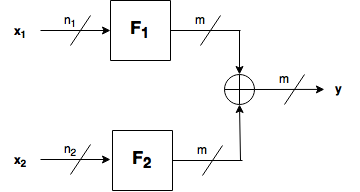
\includegraphics{DirectSum}
\caption[Direct Sum]{\textit{Direct Sum}.}
\label{fig:DirectSum}
\end{figure}

\subsection{Library}

The method included in VBF to perform this construction is the following:

\begin{verbatim}
void directsum(VBF& X, VBF& F, VBF& G)  
\end{verbatim}

\begin{example}
The following program provides the weight, algebraic degree, balancedness, correlation immunity, nonlinearity and algebraic immunity of two Vector Boolean functions given its polynomial representation in ANF and calculates the same criteria for the its direct sum.

\begin{verbatim}
#include <iostream>
#include <fstream>
#include "VBF.h"

int main(int argc, char *argv[])
{
   using namespace VBFNS;

   VBF          F, G, X;

   ifstream input1(argv[1]);
   if(!input1){
      cerr << "Error opening " << argv[1] << endl;
      return 0;
   }
   F.putHexTT(input1);
   input1.close();

   ifstream input2(argv[2]);
   if(!input2) {
      cerr << "Error opening " << argv[2] << endl;
      return 0;
   }
   G.putHexTT(input2);
   input2.close();

   cout << "weight(F)=" << weight(F) << endl;
   cout << "deg(F)=" << deg(F) << endl;
   if (Bal(F)) {
     cout << "F is a balanced function" << endl;
   } else {
     cout << "F is a non-balanced function" << endl;
   }
   cout << "Degree of Correlation immunity of F=" << CI(F) << endl;
   cout << "R(F)=" << SpectralRadius(F) << endl;
   cout << "nl(F)=" << nl(F) << endl;
   cout << "ACmax(F)=" << maxAC(F) << endl;
   cout << "ld(F)=" << ld(F) << endl;
   cout << "AI(F)=" << AI(F) << endl;
   cout << "F is PC of degree " << PC(F) << endl;
   cout << endl;

   cout << "weight(G)=" << weight(G) << endl;
   cout << "deg(G)=" << deg(G) << endl;
   if (Bal(G)) {
     cout << "G is a balanced function" << endl;
   } else {
     cout << "G is a non-balanced function" << endl;
   }
   cout << "Degree of Correlation immunity of G=" << CI(G) << endl;
   cout << "R(G)=" << SpectralRadius(G) << endl;
   cout << "nl(G)=" << nl(G) << endl;
   cout << "ACmax(G)=" << maxAC(G) << endl;
   cout << "ld(G)=" << ld(G) << endl;
   cout << "AI(G)=" << AI(G) << endl;
   cout << "G is PC of degree " << PC(G) << endl;
   cout << endl;

   directsum(X,F,G);

   cout << "weight(F directsum G)=" << weight(X) << endl;
   cout << "deg(F directsum G)=" << deg(X) << endl;
   if (Bal(X)) {
     cout << "F directsum G is a balanced function" << endl;
   } else {
     cout << "F directsum G is a non-balanced function" << endl;
   }
   cout << "Degree of Correlation immunity of F directsum G=" << CI(X) << endl;
   cout << "R(F directsum G)=" << SpectralRadius(X) << endl;
   cout << "nl(F directsum G)=" << nl(X) << endl;
   cout << "ACmax(F directsum G)=" << maxAC(X) << endl;
   cout << "ld(F directsum G)=" << ld(G) << endl;
   cout << "AI(F directsum G)=" << AI(X) << endl;
   cout << "F directsum G is PC of degree " << PC(X) << endl;

   return 0;
}
\end{verbatim}

If we use the Boolean functions with the following Truth Tables (in hexadecimal representation) as inputs:

\begin{verbatim}
6cb405778ea9bd30
\end{verbatim}

\begin{verbatim}
5c721bcaac27b1c5
\end{verbatim}

The output would be the following:

\begin{verbatim}
weight(F)=32
deg(F)=3
F is a balanced function
Degree of Correlation immunity of F=1
R(F)=16
nl(F)=24
ACmax(F)=32
ld(F)=8
AI(F)=3
F is PC of degree 2

weight(G)=32
deg(G)=3
G is a balanced function
Degree of Correlation immunity of G=2
R(G)=32
nl(G)=16
ACmax(G)=64
ld(G)=0
AI(G)=2
G is PC of degree 1

weight(F directsum G)=2048
deg(F directsum G)=3
F directsum G is a balanced function
Degree of Correlation immunity of F directsum G=4
R(F directsum G)=512
nl(F directsum G)=1792
ACmax(F directsum G)=4096
ld(F directsum G)=0
AI(F directsum G)=3
F directsum G is PC of degree 1
\end{verbatim}

These results are congruent with the properties derived in \cite{SarkarMaitra:00} and others derived by Jose Antonio Alvarez:

\begin{itemize}
\item $wt(F \oplus G) = 2^6 \cdot 32+2^6 \cdot 32 - 2 \cdot 32 \cdot 32 = 2048$.

\item $\crit{deg}(F \oplus G) = \max \left\{ 3, 3 \right\} = 3$.

\item $F$ is $1$-resilient, $G$ is $2$-resilient, and $F \oplus G$ is $(1+2+1)$-resilient.

\item $\crit{R}(F \oplus G) = 16 \cdot 32=512$ because $F$ and $G$ are Boolean functions.

\item $\crit{NL}(F \oplus G) = 2^{12-1} -\frac{1}{2} \cdot 512 = 1792$.

\item $\crit{AC_{max}}(F \oplus G) = \max \{ 32 \cdot 64, 64 \cdot 64 \} = 4096$.

\item $\crit{LD}(F \oplus G) =2^{12-2}-\frac{1}{4} \cdot 4096 = 0$.

\item $\max \{ 3, 2 \} \leq \crit{AI}(F \oplus G) = 3 \leq \min \left\{ \max \left\{ 3 , 3 \right\} ,  3 + 2 \right\}$.

\end{itemize}
\end{example}

\section{Concatenation}

\subsection{Description}

\begin{definition}
Let $n_1,n_2 \geq 1$, $F_1 \in \funct{F}_{n,m}, F_2 \in \funct{F}_{n,m}$ be Vector Boolean functions. Consider the Vector Boolean function $F_1 |_{c} F_2 \in \funct{F}_{n+1,m}$ defined as $(\vec{x},x_{n+1}) \rightarrow \left( x_{n+1}+1 \right) F_1(\vec{x})+ x_{n+1} F_2(\vec{x})$ where $\vec{x} \in \gf{V_n}$.
\end{definition}

\subsection{Library}

The method included in VBF to perform this construction is the following:

\begin{verbatim}
void concat(VBF& X, VBF& F, VBF& G)  
\end{verbatim}

\begin{example}
The following program provides the weight, algebraic degree, balancedness, correlation immunity, nonlinearity and algebraic immunity of two Vector Boolean functions given its polynomial representation in ANF and calculates the same criteria for its concatenation.

\begin{verbatim}
#include <iostream>
#include <fstream>
#include "VBF.h"

int main(int argc, char *argv[])
{
   using namespace VBFNS;

   VBF          F, G, X;
   vec_pol f,g;

   ifstream input1(argv[1]);
   if(!input1) {
      cerr << "Error opening " << argv[1] << endl;
      return 0;
   }
   input1 >> f;
   F.putpol(f);
   input1.close();

   ifstream input2(argv[2]);
   if(!input2) {
      cerr << "Error opening " << argv[2] << endl;
      return 0;
   }
   input2 >> g;
   G.putpol(g);
   input2.close();

   cout << "weight(F)=" << weight(F) << endl;
   cout << "deg(F)=" << deg(F) << endl;
   if (Bal(F))  {
     cout << "F is a balanced function" << endl;
   } else {
     cout << "F is a non-balanced function" << endl;
   }
   cout << "Degree of Correlation immunity of F=" << CI(F) << endl;
   cout << "nl(F)=" << nl(F) << endl;
   cout << "AI(F)=" << AI(F) << endl;
   cout << endl;

   cout << "weight(G)=" << weight(G) << endl;
   cout << "deg(G)=" << deg(G) << endl;
   if (Bal(G)) {
     cout << "G is a balanced function" << endl;
   } else {
     cout << "G is a non-balanced function" << endl;
   }
   cout << "Degree of Correlation immunity of G=" << CI(G) << endl;
   cout << "nl(G)=" << nl(G) << endl;
   cout << "AI(G)=" << AI(G) << endl;
   cout << endl;

   concat(X,F,G);
   cout << "The polynomial in ANF of the concatenation of F and G is ";
   cout << endl;
   Pol(cout,X);

   cout << "weight(F concat G)=" << weight(X) << endl;
   cout << "deg(F concat G)=" << deg(X) << endl;
   if (Bal(X)) {
     cout << "F concat G is a balanced function" << endl;
   } else {
     cout << "F concat G is a non-balanced function" << endl;
   }
   cout << "Degree of Correlation immunity of F concat G=" 
   << CI(X) << endl;
   cout << "nl(F concat G)=" << nl(X) << endl;
   cout << "AI(F concat G)=" << AI(X) << endl;

   return 0;
}
\end{verbatim}

If we use the Boolean functions $1+x_3x_4+x_2+x_2x_4+x_1+x_1x_3+x_1x_3x_4$ and $x_3+x_2x_4+x_1+x_1x_4+x_1x_3x_4$ as inputs, the output would be the following:

\begin{verbatim}
weight(F)=8
deg(F)=3
F is a balanced function
Degree of Correlation immunity of F=0
nl(F)=4
AI(F)=2

weight(G)=8
deg(G)=3
G is a balanced function
Degree of Correlation immunity of G=0
nl(G)=4
AI(G)=2

The polynomial in ANF of the concatenation of F and G is
1+x4x5+x3+x3x5+x2+x2x4+x2x4x5
weight(F concat G)=16
deg(F concat G)=3
F concat G is a balanced function
Degree of Correlation immunity of F concat G=0
nl(F concat G)=8
AI(F concat G)=2
\end{verbatim}

These results are congruent with the properties of this construction:

\begin{itemize}
\item $wt(F |_{c} G) = 8 + 8 = 16$.

\item $\crit{deg}(F |_{c} G) = 3 \leq 1 + \max \left\{ 3, 3 \right\} = 1+3=4$.

\item $F$ is $0$-resilient, $G$ is $0$-resilient, and $F |_{c}  G$ is $0$-resilient.

\item $\crit{NL}(F |_{c} G) =8 \geq 4 + 4 = 8$.

\item If $\crit{AI}(F) = \crit{AI}(G) = 2$, then $\crit{AI}(F |_{c} G) = 2 \leq 2 + 1$.

\end{itemize}
\end{example}

\section{Concatenation of Polynomials in ANF}

\subsection{Description}

\begin{definition}
Let $n_1,n_2 \geq 1$, $F_1 \in \funct{F}_{n_1,m}, F_2 \in \funct{F}_{n_2,m}$ be Vector Boolean functions. Consider the Vector Boolean function $F_1 |_{p} F_2 \in \funct{F}_{n_1+n_2,m}$ defined as $(x_1,\ldots,x_{n_1},x_{n_1+1},\ldots,x_{n_1+n_2}) \rightarrow F_1(x_1,\ldots,x_{n_1})+ F_2(x_{n_1+1},\ldots,x_{n_1+n_2})$ where $\vec{x} \in \gf{V_{n_1+n_2}}$.
\end{definition}

\subsection{Library}

The method included in VBF to perform this construction is the following:

\begin{verbatim}
void concatpol(VBF& X, VBF& F, VBF& G)  
\end{verbatim}

\begin{example}
The following program provides the ANF of the concatenation of polynomials in ANF of two Vector Boolean functions given its polynomial representation.

\begin{verbatim}
#include <iostream>
#include <fstream>
#include "VBF.h"

int main(int argc, char *argv[])
{
   using namespace VBFNS;

   VBF          F,G,H;
   vec_pol     f,g;
   NTL::mat_GF2 T;

   ifstream inputf(argv[1]);
   if(!inputf) {
      cerr << "Error opening " << argv[1] << endl;
      return 0;
   }
   inputf >> f;
   F.putpol(f);
   inputf.close();

   ifstream inputg(argv[2]);
   if(!inputg) {
      cerr << "Error opening " << argv[2] << endl;
      return 0;
   }
   inputg >> g;
   G.putpol(g);
   inputg.close();

   concatpol(H,F,G);
   cout << "The ANF of the concatenation of polynomials 
   in ANF of F and G is ";
   cout << endl;
   Pol(cout,H);

   return 0;
}

\end{verbatim}

If we use the Boolean functions $x_1x_2+x_3x_4$ and $x_1+1$ as inputs, the output would be the following:

\begin{verbatim}
The ANF of the concatenation of polynomials in ANF of F and G is 
x1x2+x3x4+x5+1
\end{verbatim}

\end{example}

\section{Addition of Coordinate Functions}

\subsection{Description}

\begin{definition}
Let $F=(f_1,\ldots,f_{m_1}) \in \funct{F}_{n,m_1}$, $G=(g_1,\ldots,g_{m_2}) \in \funct{F}_{n,m_2}$ and the function conformed by adding the coordinate functions $(F,G) =(f_1,\dots,f_{m_1},g_1,\ldots,g_{m_2}) \in \funct{F}_{n,m_1+m_2}$. Let $\vec{v} \in \gf{V_{m_1+m_2}}$,$\vec{v_F} \in \gf{V_{m_1}}$ and $\vec{v_G} \in \gf{V_{m_2}}$ so that $\vec{v} = (\vec{v_F}, \vec{v_G})$. See figure~\ref{fig:AddImage}.
\end{definition}

\begin{figure}[htbp!]
\centering
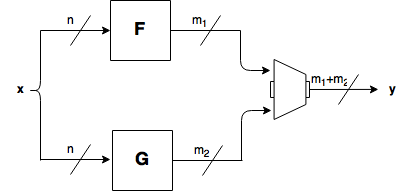
\includegraphics{AddImage}
\caption[Adding Coordinate functions]{\textit{Adding Coordinate functions}.}
\label{fig:AddImage}
\end{figure}

\subsection{Library}

This construction can be obtained with the following method:

\begin{verbatim}
void addimage(VBF& X, VBF& F, VBF& G)  
\end{verbatim}

\begin{example}\label{CLEFIA:AddCoordinate}
The following program provides the Truth Tables of the different intermediate constructions that allow to obtain CLEFIA $S_0$ $8 \times 8$ S-box from the Truth Tables of the four 4-bit S-boxes $SS_0,SS_1,SS_2$ and $SS_3$ in which it is constructed and the Truth Table of the multiplication operation in $0x2$ performed in $\gf{GF(2^4)}$ defined by the
primitive polynomial $x^4 + x + 1$. 

\begin{verbatim}
#include <iostream>
#include <fstream>
#include "VBF.h"

int main(int argc, char *argv[])
{
   using namespace VBFNS;

   VBF F,G,T20,T21,U0,U1,Y0,Y1,Y;
   NTL::mat_GF2 TSS0, TSS1, TSS2, TSS3, Tmul2;
   NTL::mat_GF2 T2t0, T2t1, Tu0, Tu1, Ty0, Ty1, Ty;

   ifstream inputSS0("SS0.tt");
   if(!inputSS0) {
      cerr << "Error opening " << "SS0.tt" << endl;
      return 0;
   }
   inputSS0 >> TSS0;
   inputSS0.close();

   ifstream inputSS1("SS1.tt");
   if(!inputSS1) {
      cerr << "Error opening " << "SS1.tt" << endl;
      return 0;
   }
   inputSS1 >> TSS1;
   inputSS1.close();

   ifstream inputSS2("SS2.tt");
   if(!inputSS2) {
      cerr << "Error opening " << "SS2.tt" << endl;
      return 0;
   }
   inputSS2 >> TSS2;
   inputSS2.close();

   ifstream inputSS3("SS3.tt");
   if(!inputSS3) {
      cerr << "Error opening " << "SS3.tt" << endl;
      return 0;
   }
   inputSS3 >> TSS3;
   inputSS3.close();

   ifstream inputmul2("Mul2.tt");
   if(!inputmul2) {
      cerr << "Error opening " << "Mul2.tt" << endl;
      return 0;
   }
   inputmul2 >> Tmul2;
   inputmul2.close();

   cout << "t0=" << endl;
   cout << TSS0 << endl << endl;
   cout << "t1=" << endl;
   cout << TSS1 << endl << endl;
   F.puttt(TSS1);
   G.puttt(Tmul2);
   Comp(T21,F,G);
   T2t1 = TT(T21);
   cout << "0x2.t1=" << endl;
   cout << T2t1 << endl;
   F.kill();
   G.kill();
   F.puttt(TSS0);
   G.puttt(Tmul2);
   Comp(T20,F,G);
   T2t0 = TT(T20);
   cout << "0x2.t0=" << endl;
   cout << T2t0 << endl;
   cout << "u0=t0+0x2.t1=" << endl;
   F.kill();
   F.puttt(TSS0);
   directsum(U0,F,T21);
   Tu0 = TT(U0);
   cout << Tu0 << endl;
   G.kill();
   cout << "u1=0x2.t0+t1=" << endl;
   G.puttt(TSS1);
   directsum(U1,T20,G);
   Tu1 = TT(U1);
   cout << Tu1 << endl;
   G.kill();
   cout << "y0=SS2(u0)=" << endl;
   G.puttt(TSS2);
   Comp(Y0,U0,G);
   Ty0 = TT(Y0);
   cout << Ty0 << endl;
   G.kill();
   cout << "y1=SS3(u1)=" << endl;
   G.puttt(TSS3);
   Comp(Y1,U1,G);
   Ty1 = TT(Y1);
   cout << Ty1 << endl;
   addimage(Y,Y0,Y1);
   Ty = TT(Y);
   cout << "y=(y0,y1)=" << endl;
   cout << Ty << endl;

   return 0;
}
\end{verbatim}

The output of this program is described in section "Analysis of CRYPTEC project cryptographic algorithms".

Note that the output of $S_0$ S-box $\vec{y} \in \funct{F}_{8,8}$ is defined by the addition of coordinate functions of both $\vec{y_0} \in \funct{F}_{8,4}$ and $\vec{y_1} \in \funct{F}_{8,4}$. 
\end{example}

\section{Bricklayer}

\subsection{Description}

\begin{definition}
Let $n_1,n_2,m_1,m_2 \geq 1$ and $F_1 \in \funct{F}_{n_1,m_1}$ , $F_2 \in \funct{F}_{n_2,m_2}$ and the Bricklayer function $F_1 | F_2 \in \funct{F}_{n_1+n_2,m_1+m_2}$. Let $\vec{u_1} \in \gf{V_{n_1}}$, $\vec{u_2} \in \gf{V_{n_2}}$ and $\vec{u}=(\vec{u_1} , \vec{u_2})$, $\vec{v_1} \in \gf{V_{m_1}}$, $\vec{v_2} \in \gf{V_{m_2}}$ and $\vec{v}=(\vec{v_1} , \vec{v_2})$.  See figure~\ref{fig:Bricklayer}.
\end{definition}

\begin{figure}[htbp!]
\centering
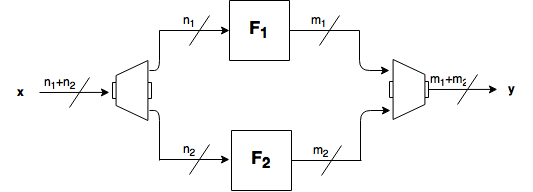
\includegraphics[width=\textwidth]{Bricklayer}
\caption[Bricklayer]{\textit{Bricklayer}.}
\label{fig:Bricklayer}
\end{figure}

\subsection{Library}

It can be obtained with the following method:
     
\begin{verbatim}
void bricklayer(VBF& X, VBF& F, VBF& G)  
\end{verbatim}

\begin{example}
KHAZAD is a block cipher designed by Paulo S. L. M. Barreto together with Vincent Rijmen, which was presented at the first NESSIE workshop in 2000, and, after some small changes, was selected as a finalist in the project. This cipher uses a $8 \times 8$ S-box composed of smaller pseudo-randomly generated $4 \times 4$  mini S-boxes (the P-box and the Q-box) as represented in figure~\ref{fig:KHAZADS}.

\begin{figure}[htbp!]
\centering
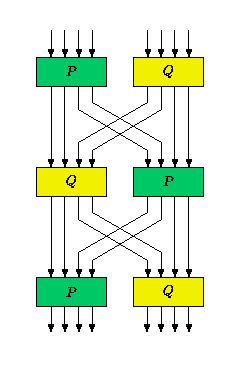
\includegraphics[width=\textwidth]{KHAZADS}
\caption[KHAZAD S-box construction]{\textit{KHAZAD S-box construction}.}
\label{fig:KHAZADS}
\end{figure}

The following program provides the Truth Tables of the different intermediate constructions that allow to obtain KHAZAD S-box from $P$ and $Q$ mini S-boxes and the permutation that apply between them.

\begin{verbatim}
#include <iostream>
#include <fstream>
#include "VBF.h"

int main(int argc, char *argv[])
{
   using namespace VBFNS;

   VBF          P, Q, PQ, R, QP, S, T, U, A;
   NTL::mat_GF2 Tp, Tq;
   NTL::vec_ZZ  r;

   ifstream inputp("P.tt");
   if(!inputp) {
      cerr << "Error opening " << "P.tt" << endl;
      return 0;
   }
   inputp >> Tp;
   P.puttt(Tp);
   inputp.close();

   ifstream inputq("Q.tt");
   if(!inputq) {
      cerr << "Error opening " << "Q.tt" << endl;
      return 0;
   }
   inputq >> Tq;
   Q.puttt(Tq);
   inputq.close();

   ifstream input("R.per");
   if(!input)  {
      cerr << "Error opening " << "R.per" << endl;
      return 0;
   }
   input >> r;
   R.putper(r);
   input.close();

   bricklayer(PQ,P,Q);
   cout << "Bricklayer of P and Q=" << endl;
   cout << TT(PQ) << endl;
   
   Comp(S,PQ,R);
   cout << "Composition of 1st bricklayer 
   with permutation=" << endl;
   cout << TT(S) << endl;

   bricklayer(QP,Q,P);
   cout << "Bricklayer of Q and P=" << endl;
   cout << TT(QP) << endl;

   Comp(T,S,QP);
   cout << "Composition of previous result 
   with 2nd bricklayer=" << endl;
   cout << TT(T) << endl;

   Comp(U,T,R);
   cout << "Composition of previous result 
   with permutation=" << endl;
   cout << TT(U) << endl;

   Comp(A,U,PQ);
   cout << "Composition of previous result 
   with 1st bricklayer=" << endl;
   cout << TT(A) << endl;

   return 0;
}
\end{verbatim}

If we use the Truth Tables of $P$ and $Q$ and the representation of the permutation between them, the output are the Truth Tables described KHAZAD section in "Analysis of NESSIE project cryptographic algorithms".

\begin{table}[htbp]
\caption{Results of spectral radius($\crit{r}$),$\crit{NL}, \crit{lp}, \crit{dp}, \crit{AC_{max}}$ and $\crit{LD}$ for bricklayer of $P$ and $Q$ mini S-boxes.}
\centering
\label{tab:Khazad}
\begin{tabular}{ l l l l l l l }
\toprule
S-box & $\crit{r}$ & $\crit{NL}$ & $\crit{lp}$ & $\crit{dp}$ & $\crit{AC_{max}}$ & $\crit{LD}$ \\
\midrule
$P$ & $8$ & $4$ & $0.25$ & $0.25$ & $8$ & $2$ \\
$Q$ & $8$ & $4$ & $0.25$ & $0.25$ & $8$ & $2$ \\
$P | Q$ & $128$ & $64$ & $0.25$ & $0.25$ & $256$ & $0$ \\
$Q | P$ & $128$ & $64$ & $0.25$ & $0.25$ & $256$ & $0$ \\
$R \circ (P | Q)$ & $128$ & $64$ & $0.25$ & $0.25$ & $256$ & $0$ \\
%$R \circ (P | Q)$ & $128$ & $64$ & $0.25$ & $0.25$ & $256$ & $0$ \\
$(Q|P) \circ \left( \left( R \circ (P | Q) \right) \right)$ & $96$ & $80$ & $0.140625$ & $0.125$ & $160$ & $24$ \\
$R \circ \left( (Q|P) \circ \left( \left( R \circ (P | Q) \right) \right) \right)$ & $96$ & $80$ & $0.140625$ & $0.125$ & $160$ & $24$ \\
$S = (P|Q) \circ \left( R \circ \left( (Q|P) \circ \left( \left( R \circ (P | Q) \right) \right) \right) \right)$ & $64$ & $96$ & $0.0625$ & $0.03125$ & $104$ & $38$ \\
\bottomrule
\end{tabular}
\end{table}

\end{example}

\begin{example}
The following program provides the balancedness and correlation immunity (resiliency) of two Vector Boolean functions given its Truth Table in hexadecimal representation and calculates the same criteria for the bricklayering of $F$ and $G$ taking as inputs their Truth Tables in hexadecimal representation.

\begin{verbatim}
#include <iostream>
#include <fstream>
#include "VBF.h"

int main(int argc, char *argv[])
{
   using namespace VBFNS;

   VBF          F, G, H;

   ifstream input1(argv[1]);
   if(!input1) {
      cerr << "Error opening " << argv[1] << endl;
      return 0;
   }
   F.putHexTT(input1);
   input1.close();

   ifstream input2(argv[2]);
   if(!input2) {
      cerr << "Error opening " << argv[2] << endl;
      return 0;
   }
   G.putHexTT(input2);
   input2.close();

   cout << "Correlation immunity of F: " << CI(F) << endl;
   if (Bal(F)) {
     cout << "F is a balanced function" << endl;
   } else {
     cout << "F is a non-balanced function" << endl;
   }

   cout << "Correlation immunity of G: " << CI(G) << endl;
   if (Bal(G)) {
     cout << "G is a balanced function" << endl;
   } else {
     cout << "G is a non-balanced function" << endl;
   }

   bricklayer(H,F,G);

   cout << "Correlation immunity of F bricklayer G: " << CI(H) << endl;
   if (Bal(H)) {
     cout << "F bricklayer G is a balanced function" << endl;
   } else {
     cout << "F bricklayer G is a non-balanced function" << endl;
   }

   return 0;
}
\end{verbatim}

If we use the Boolean functions with the following Truth Tables (in hexadecimal representation) as inputs:

\begin{verbatim}
6cb405778ea9bd30
\end{verbatim}

\begin{verbatim}
5c721bcaac27b1c5
\end{verbatim}

The output would be the following:

\begin{verbatim}
Correlation immunity of F: 1
F is a balanced function
Correlation immunity of G: 2
G is a balanced function
Correlation immunity of F bricklayer G: 1
F bricklayer G is a balanced function
\end{verbatim}

\end{example}

\section{Summary}

Table~\ref{tab:Operations} lists the member functions related to the
previous characterizing elements.

\begin{table}[htbp]
\caption{Constructions over VBF.}
\centering
\label{tab:Operations}
\begin{tabular}{ l l }
\toprule
SYNTAX & DESCRIPTION \\
\midrule
\textit{long operator==(VBF\& F, VBF\& G)} & Returns $1$ if $F$ and $G$ are equal \\
& 0 otherwise \\
\textit{void Comp(VBF\& X, VBF\& F, VBF\& G)} & $X = G \circ F$ \\
\textit{void inv(VBF\& X, VBF\& A)} & $X = F^{-1}$ \\
\textit{void sum(VBF\& X, VBF\& F, VBF\& G)} & $X = F+G$ \\
\textit{void directsum(VBF\& X, VBF\& F, VBF\& G)} & $X(\vec{x},\vec{y}) = F(\vec{x}) + G(\vec{y})$ \\
\textit{void concat(VBF\& X, VBF\& F, VBF\& G)} & $X(\vec{x},x_{n+1}) =\left( x_{n+1}+1 \right) F(\vec{x})+ x_{n+1} G(\vec{x})$ \\
\textit{void concatpol(VBF\& X, VBF\& F, VBF\& G)} & $X(x_1,\ldots,x_{n_1},x_{n_1+1},\ldots,x_{n_1+n_2})$ \\
& $= F(x_1,\ldots,x_{n_1})+G(x_{n_1+1},\ldots,x_{n_1+n_2})$ \\
\textit{void addimage(VBF\& X, VBF\& F, VBF\& G)} & $X = (F,G)$ \\
\textit{void bricklayer(VBF\& X, VBF\& F, VBF\& G)} & $X = F | G$ \\
\bottomrule
\end{tabular}
\end{table}
